%!TEX root = ../main.tex

\chapter{Theoretical Framework}
\label{chp:theoreticalFramework}

\section{Deposit-Refund System for Bottled Beverages in Germany}
\subsection{Legal Basis}
\label{sec:legalBasis}
Anticipating the depletion of capacity in disposal sites and due to the considerable share in waste generated by packaging \footnote{Recycling rate of packaging was below 50\% in the early 1990s (20\% for aluminium and plastic) \hide{\cite{GVM2010}} \cite[p.~2]{Hartlep2011Recycling}.} \cite[p.~2]{Hartlep2011Recycling}, German federal government enacted an ordinance regarding the avoidance of packaging waste (\textit{Verordnung über die Vermeidung von Verpackungsabfällen}, short: \textit{\ac{VerpackV}}) in 1991 which stipulates that packaging \cite[§~1]{verpackV1991}:

\begin{itemize}
  \item must be minimised to an extent necessary for protection and marketing of goods
  \item must be reused where possible
  \item must be recycled if reuse is not applicable 
\end{itemize}

These objectives were supported by introducing the:

\begin{description}
	\item[Obligation to take back packaging]
	\hfill \\
	Producers and distributors of packaging are obliged to take back packaging free of charge, restricted to those goods of type, shape, size and material found within their stock \cite[§§~4-6]{verpackV1991}. Distributors with a retail area of less than 200$m^2$ are further exempted to the same brands. This duty may be only be ignored if a distributor participates in a system which ensures the periodical collection of waste \cite[§~6]{verpackV1991}, known and implemented as a refuse recycling system (\textit{duales System}) in 1990 \cite[p.~3]{Hartlep2011Recycling}.
	\item[Obligation to levy deposits on \gls{beverage packaging}] \footnote{Information regarding the assumed effects and critique thereof can be found in \cite[p.~630]{Cora2000} and \cite{wacker2008pflichtpfand}.}
	\hfill \\
	A deposit is to be charged by the distributor that will be refunded to the purchaser upon return of the bottle. This duty is applicable on all levels of trade involving domestic beverages sold in non-\gls{reusable packaging} (\textit{one-way packaging}) \cite[§~7]{verpackV1991} and becomes effective as soon as the quote of reusable beverage packaging falls below 72\% \footnote{Aggregated quote derived from weighted average of percentages of reusable packaging encountered across individual segments in 1990 \cite[§~9]{verpackV1991} \cite[p.~134]{Rummler/Schutt1991}} \cite[§~9]{verpackV1991}.
\end{description}

%\todo[inline]{figure showcasing development of aggregated reusable packaging quote}
%\todo[inline]{explain highs and separation of dataset}

\begin{figure}[hbt]
	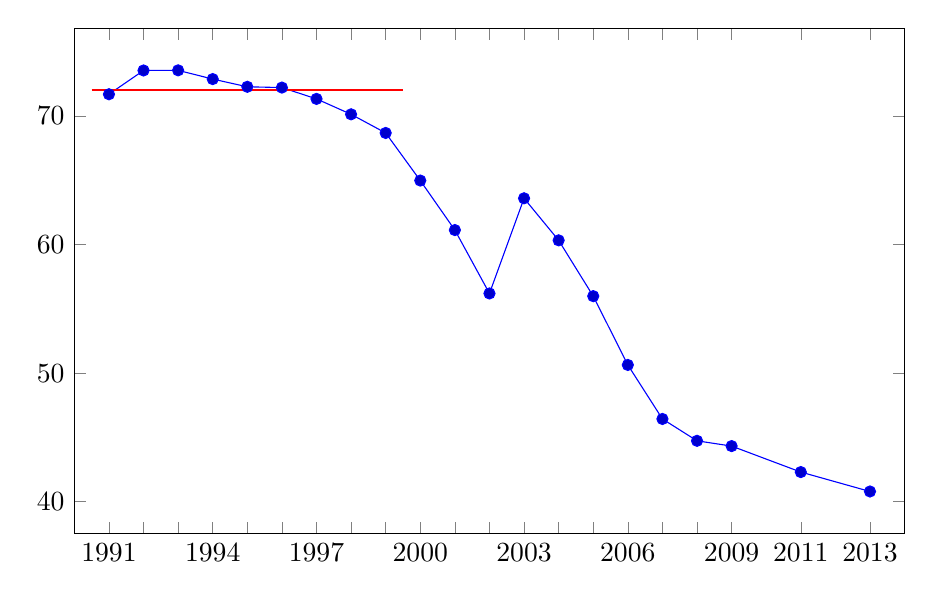
\begin{tikzpicture}
        \begin{axis}[
%            xlabel = Lines to process (\#),
%            ylabel = Execution time (seconds),
			xtick = data,
			xticklabels={1991, , , 1994, , , 1997, , , 2000, , , 2003, , , 2006, , , 2009, 2011, 2013},
			height = 8cm,
            width =\textwidth,
%            legend pos = north west,
%            title = {File Processing Speeds~\footnotemark}
			xmin=0,
			xmax=24,
		]
	
        \addplot+[sharp plot, color=blue]
            coordinates {
                (1, 71.69) (2, 73.54) (3, 73.55) (4, 72.87) (5, 72.27) (6, 72.21) (7, 71.33)
                (8, 70.13) (9, 68.68) (10, 64.98)
                (11, 61.13) (12, 56.2) (13, 63.6) (14, 60.33) (15, 55.99) (16, 50.64)
                (17, 46.44) (18, 44.74) (19, 44.33) (21, 42.31) (23, 40.8)
                
%                (20, 48) (21, 48) (22, 45.7) (23, 45.1) (24, 45.1) (25, 44.3) 
            };
        
        \addplot[mark=none, thick, red, domain=0.5:9.5] {72};
        
		\end{axis}
	\end{tikzpicture}
  	\caption{Aggregated quote of reusable beverage packaging between 1991 and 2013 \cite[p.~1]{BMU2015} \hide{\cite{statista2015Mehrweg}}}
  	\label{fig:reusableQuoteDevelopment}
\end{figure}

Starting in 1997, the threshold to levy deposits has been surpassed steadily (comp. \autoref{fig:reusableQuoteDevelopment}), requiring an additional assessment of the situation to ensure that the fluctuation does not represent a short-term development \cite[§ 9]{verpackV1991} \cite[p.~5]{Hartlep2011Recycling}. Although obvious at glance, the outcome of a compulsory deposit-refund system only became official on July 2\textsuperscript{nd}, 2002 \cite[p.~49]{Geyer/Smoltczyk2003}, after a lawsuit lead by multiple bottlers and distributors had delayed the initial announcement \cite{spon2011handel}. Introduction of this mandatory system was scheduled for Jan 1\textsuperscript{st}, 2003 \cite[p.~53]{Geyer/Smoltczyk2003}.

\subsection{Amendments}
The German packaging ordinance underwent several revisions, including a change of title to highlight the importance of recycling \cite{verpackV1998}. In the following, the most important changes affecting the current state (see \autoref{fig:depositCriteria}) shall be highlighted.

\begin{description}
	\item[1998]
	\hfill \\
	Trims deposit obligation to those beverages for which the quote of reusable packaging has fallen when compared to 1991, though still necessitates that overall aggregated quote undercuts threshold of 72\% \cite[pp.~142]{Flanderka1999}. Even though all five segments (beer, mineral water, carbonated soft drinks, fruit juice/non-carbonated soft drinks and wine) have failed this comparison \cite[p.~1]{BMU2015}, juices/non-carbonated soft drinks and wine are exempted because their decline and market volume has not been regarded significant enough to justify the costs introduced with such a system \hide{\cite[pp.~1]{BMU 2002}} \cite[pp.~6,~9]{Hartlep2011Recycling}. 
	
\todo[inline]{figure showcasing development of reusable packing quote in each segment (appendix)}

	\item[2005]
	\hfill \\
	Reduces different deposit classifications to single deposit worth \EUR{0.25} valid for all applicable beverages with a filling volume between 0.1 - 3.0 litres. Furthermore, \gls{ecologically advantageous packaging} is admitted the same treatment and classification as that of reusable packaging which represents an important shift of thought since the sole utilisation of packaging has been considered inferior to its reuse with regard to all ecological aspects \hide{\cite[p.~1]{BMU 2010c}} \cite[p.~7]{Hartlep2011Recycling}. Accordingly, the new goal is to promote the use of ecologically advantageous packaging with a target of 80\% market dominance \cite[§~1]{verpackV2008}. This amendment also adds non-carbonated soft drinks and mixed alcoholic drinks to the list of beverages subject to deposits (irrespective of the reusable packaging quote experienced) while simultaneously protecting dietary products from deposits \cite[p.~1408]{verpackV2005} \cite[p.~171]{Flanderka/Stroetmann2009}. Finally, retailers are required to take back any bottles made from a beverage packaging material (glas, metal, paper and plastic) also sold by that store (brand equality for retail areas of less than 200$m^2$ still applies) \hide{\cite[p.~1]{BMU 2010c}}\hide{\cite[p.~7]{BMU 2010b}} \cite[p.~11]{Hartlep2011Recycling}. Previously, return had been limited to bottles of same shape, size [..] and type (comp. \ref{sec:legalBasis}). This regulation attempts to stop isolated deposit-refund systems which arose because discounters created their own specially shaped bottles \cite[p.~168]{Flanderka/Stroetmann2009}. To conform with this change, industry and commerce established the \acl{DPG}, responsible for setting up a nationwide deposit-refund system \hide{\cite[p.~1]{BMU 2010c}} \cite[p.~8]{Hartlep2011Recycling}.
	
	\item[2008]
	\hfill \\
	Orders distributors to clearly mark bottles as being obliged to a deposit. Further, distributors are demanded to participate in a nationwide deposit-refund system to enable the mutual settlement of claimed deposits \cite[§~9]{verpackV2008}. Lastly, the exemption for dietary products is reduced to infant nutrition. This acts as a measure to counteract increasingly false product declarations attempting to forego deposits \cite[pp.~531]{verpackV2008} \cite[p.~171]{Flanderka/Stroetmann2009}.
\end{description}

\todo[inline, color=orange]{add 2019 amendment}
%\todo[inline]{figure showcasing current situation}

\begin{figure}[hbt]
	\centering
	\includegraphics{images/one_way_packaged_beverages_deposit_criteria}
	\caption{Criteria to be considered for deposits (valid until Jan 1\textsuperscript{st}, 2019) \cite[p.~9]{Hartlep2011Recycling}}
	\label{fig:depositCriteria}
\end{figure}

\FloatBarrier

\subsection{Operation}

\subsubsection{Administration by \acl{DPG}}
\ac{VerpackV} simply assumes that a nationwide deposit-refund system will be installed by May 1\textsuperscript{st}, 2006 without further specifying its exact implementation details \cite[Art.~2]{verpackV2005} \cite[§~9]{verpackV2008}. Therefore, \ac{DPG} has been founded in 2005 to ensure the definition of a standards framework, which includes IT-processes, APIs and a universal security mark identifying one-way packaged bottles on which a deposit is paid (\textit{returnable bottle}). Other tasks concern the management of contracts, certifications and maintenance of a centralised database which stores information about products, participants and reverse vending machines \cite[pp.~13]{Hartlep2011Recycling}\hide{\cite[pp.~96]{DPG/Roland Berger 2010}}. However, \ac{DPG} does not have access to purchasing data (e.g. number of sold and returned bottles or total amount of reimbursed deposits). This data is only exchanged between actors of the deposit-refund cycle. Consequently, \ac{DPG} is not involved in the process of settling refund claims between take-back points and does not act as a central clearing house. It is exclusively responsible for providing a contractual and administrative basis needed to enable such a system \cite[p.~14]{Hartlep2011Recycling}.

\todo[inline]{figure showcasing universal security mark (appendix)}

\subsubsection{Roles}
As indicated, actors of the deposit-refund cycle (e.g. retailer selling returnable bottles) must register with \ac{DPG}, accept the contractual basis for the role to be exercised and pay a yearly membership fee in order to participate\hide{\cite[p.~15]{Hartlep2011Recycling}}\hide{\cite[p.~34]{DPG/Roland Berger 2010}}. The most important roles are \hide{\cite[pp.~33-34]{DPG/Roland Berger 2010}} \cite[pp.~15-16]{Hartlep2011Recycling}:   

\begin{description}
	\item[Initial distributor]
	\hfill \\
	Puts returnable bottle into circulation. Inherently tied to role of deposit escrow account manager. Must pay a one-time fee to register a beverage (i.e. an \acs{EAN}) with \ac{DPG}'s central database. This fee depends on the number of pieces produced within a year for that beverage.
%	Commonly exercised by bottler or importer but may also include retailers selling their own brands.
	\item[Deposit escrow account manager]
	\hfill \\
	Administrates and disburses money received from levying deposit on returnable bottle. Task may be delegated to a service provider.
	\item[Take-back point]
	\hfill \\
	Refunds consumer in exchange for returning bottles subject to deposits. Inherently tied to role of refund claimant.
	\item[Refund claimant]
	\hfill \\
	Puts in a claim to be reimbursed for making advance refunds. Task may be delegated to a service provider.
	\item[Counting center operator]
	\hfill \\
	Takes over role of reverse vending machine by confirming number of genuinely accepted bottles with a receipt. 
	
\end{description}

\subsubsection{Deposit-Refund Cycle}
Each buyer of a returnable bottle must directly pay the designated deposit to the seller. This process starts with the initial distributor (step 1 of \autoref{fig:depositRefundCycle}) and is repeated for each sub-distributor until the bottles reaches retail which acts as the final distributor to end consumers (step 2 of \autoref{fig:depositRefundCycle}). After consumption, the consumer may return the packaging at any retail store obliged to take back the packaging in question (take-back point) (step 3 of \autoref{fig:depositRefundCycle}). Return may be performed manually (step 1a of \autoref{fig:clearingProcess}) or can be automated through reverse vending machines (step 1b of \autoref{fig:clearingProcess}). The former requires personnel to count the number of returned bottles and refund the consumer accordingly. Following count, the collected bottles must be shipped to a counting center which is responsible for digitally capturing each bottle (step 2a of \autoref{fig:clearingProcess})\hide{\cite[p.~76]{DPG/Roland Berger 2010}}\hide{\cite[p.~17]{Hartlep2011Recycling}}. At last, the bottles will be compressed to eliminate the possibility of repeated refunds\hide{\cite[p.~77]{DPG/Roland Berger 2010}}. In the case of reverse vending machines, the process of counting, capturing and compressing bottles can take place locally at a retail store (step 2b of \autoref{fig:clearingProcess})\hide{\cite[p.~76]{DPG/Roland Berger 2010}}. Alternatively, retailers are permitted to return the packaging to the previous distributor, thereby unwinding the deposit-refund chain. However, this practice is rarely exercised since the packaging will not be reused and transportation would only induce additional ecological and financial strain\hide{\cite[p.~17]{Hartlep2011Recycling}}. Instead, the compressed packaging can be sold directly to recycling companies (step 3 of \autoref{fig:clearingProcess}) \cite[p.~16-17]{Hartlep2011Recycling} \cite{reiling}.  

%\todo[inline]{figure showcasing deposit-refund cycle}

\begin{figure}[hbt]
  \includegraphics{images/deposit_cycle_current_short}
  \caption{Deposit-refund cycle \cite[p.~14]{Hartlep2011Recycling}}
  \label{fig:depositRefundCycle}
\end{figure}

Since take-back points refund consumers independent of a bottle’s purchasing location, a settlement process (\textit{clearing}) is required to reimburse retailers for making advance refunds (step 4 of \autoref{fig:depositRefundCycle}). This clearing happens by issuing a refund invoice to the initial distributor who can use the deposits originally collected the pay the bill (step 4 of \autoref{fig:clearingProcess}). Ideally, all accounts are in balance, meaning that all packaging has been returned. Otherwise, a surplus on the part of an initial distributor is to be experienced \cite[p.~17]{Hartlep2011Recycling}.

%\todo[inline]{figure showcasing manual and automated return methods}

\begin{figure}[hbt]
  \includegraphics{images/bottle_return_current}
  \caption{Clearing process for manual and automated bottle returns \cite[p.~18]{Hartlep2011Recycling}}
  \label{fig:clearingProcess}
\end{figure}

Refund invoices must also include data representing the number of bottles for which a refund was issued. This data originates from the return process in which each bottle is eventually captured. Capture refers to both validating the universal security mark printed on a bottle’s label as well as extracting the \ac{EAN} by scanning its barcode. By outfitting reverse vending machines with a network connection, looking up the \ac{EAN} in question becomes possible, thus ensuring that a deposit for the bottle has been collected beforehand\hide{\cite[pp.~2]{Wincor Nixdorf 2010}}. For each valid bottle, a signed record is then produced and stored on the machine\hide{\cite[p.~18]{Hartlep2011Recycling}}. This data must be retrieved and transmitted within one week\hide{\cite[p.~90]{DPG/Roland Berger 2010}}. Likewise, retailers receive a similar dataset when relying on a counting center\hide{\cite[p.~18]{Hartlep2011Recycling}}. Finally, any transmitted data is anonymised by removing the return location and summing up the refunds for each \ac{EAN} captured\hide{\cite[pp.~90]{DPG/Roland Berger 2010}}. Initial distributors must pay the invoice within ten business days or five-teen calendar days at the lastet \hide{\cite[p.~40]{DPG/Roland Berger 2010}} \cite[p.~18-19]{Hartlep2011Recycling}.

\todo[inline, color=orange]{explain situation surrounding deposits on reusable bottles}

%\subsection{Intentions \& Effects}
%
%\subsection{Reusable Bottles}

\pagebreak

\section{Decentralized Applications}

\subsection{History \& Raison d'Être}
Johnston's Law states that everything that can be decentralised, will be decentralised \cite{JohnstonsLaw}. Fittingly, a new model for building massively scalable, successful and profitable applications, known as \textit{\acp{dApp}}, is emerging \cite[p.~5]{Raval.2016} \cite[pp.~1-2]{Johnston2015}, suggesting that this will also become the fate of the vast majority of web software applications as those follow a centralized server-client model in which individuals directly depend on a central power to send and receive information \cite[pp.~7-8]{Raval.2016}. 

The architectural structure embodied by the web has not always been as pronounced as is these days. In its early days, people would host personal servers for others to connect to and everyone owned their data. But soon, it was recognised that one individual or group could pay for the maintenance of a server and profit from users that utilize it (eg.~Amazon Web Services) and since this was easier to the average user, both conceptually and programmatically, the transition to few centralized controlling entities started \cite[pp.~14]{Raval.2016}. 

Now, users willingly give their data to service providers in return for free usage, trusting them to not misuse or sell the data elsewhere \cite[p.~24]{Raval.2016}. However, Snowden proved that this trust can, has and will be broken as long as we entrust (encrypted) data to central entities which represent a surveillance state's dream \cite{Guardian2013} \cite[p.~25]{Raval.2016}. In addition, centralized infrastructure and services increase the chances for downtime, censorship and counterparty risk \cite[p.~23]{Antonopoulos.2018}. Drawbacks like these have attributed to the development of \acp{dApp}, first fully realized by Bitcoin \footnote{BitTorrent, as an earlier example, depends on centralized trackers for data discovery \cite[p.~26]{Raval.2016}.} as a currency \cite[p.~1]{Johnston2015} \cite[p.~1]{bitcoin}. Simultaneously, recent apps (e.g.~Uber and AirBnb) attempt to decentralize real world parts of a business by providing a central and trusted data store, foreshadowing the development of decentralized apps beyond pure finances \footnote{Supports the blockchain evolution theorem proposed in \cite{Swan.2015}.} \cite[p.~15]{Raval.2016}.

The concept of \acp{dApp} is meant to take the web to its next \footnote{Web 2.0 describes the evolution towards user-generated content, responsive interfaces and interactivity \cite[p.~34]{Antonopoulos.2018}.} natural evolution \cite[pp.~34]{Antonopoulos.2018}. Web3 represents the vision of a serverless \footnote{Not to be confused with the centralized Function-as-a-Service offerings detailed in \cite{serverlessComputing}.} internet, encouraging applications to incorporate decentralised protocols in order to put users in control of their own data, identity and destiny \cite{web3}. As global economy evolves, data will become the primary form of value \cite[p.~25]{Raval.2016}, leading \citeauthor{Raval.2016} to believe that:
~
\begin{quote}
  "[\acp{dApp}] will someday become more widely used than the world's most popular web apps." \cite[p.~5]{Raval.2016}
\end{quote}

\subsection{Definition}
Developers have different opinions on what exactly a \ac{dApp} is or which components constitute it. Some think that no central point of failure is all it takes, whereas others name more specific requirements \cite[p.~9]{Raval.2016}. The following will chronologically examine the various definitions available in order to derive one used for the remainder of this thesis. 

\subsubsection{\citeyear{EthereumWhitepaper}}
\citeauthor{EthereumWhitepaper} introduces the concept of a \ac{dApp} as part of Ethereum's white paper. A complete \ac{dApp} should consist of:

\begin{itemize}
  \item low-level business-logic components
  \item high-level graphical user interface components
\end{itemize}

He goes on to state that "the blockchain and other decentralized protocols will serve as a complete replacement for the server for the purpose of handling user-initiated requests. ... Decentralized protocols ... may be used to store the web pages themselves." \cite[p.~34]{EthereumWhitepaper}. 

This vague explanation is expanded through a consequent blog post (\citeyear{Buterin2014}) in which \citeauthor{Buterin2014} formally defines the concept as being a superset of \textit{smart-contracts} \cite{Buterin2014}:

\begin{description}
	\item[Smart-contract]
	\hfill \\
	Mechanism involving digital assets and a fixed number of parties, where some or all of the parties put assets in and assets are automatically redistributed among those parties according to a formula based on certain data that is not known at the time the contract is initiated.
	\item[Decentralized application]
	\hfill \\
	Similar to a smart-contract but with unbounded number of participants and not necessarily of financial nature.
\end{description}

\subsubsection{\citeyear{Johnston2015}}
To be considered a \ac{dApp}, \citeauthor{Johnston2015} assume that an application \cite[p.~2]{Johnston2015}:

\begin{itemize}
  \item is \textbf{open-source}, operates autonomously and adapts its protocol with user consent 
  \item stores its data and records of operation in a \textbf{public blockchain}
  \item uses a \textbf{token} necessary for accessing it and rewarding contribution of value
  \item generates its tokens according to a predefined \textbf{cryptographic algorithm}
\end{itemize}

Moreover, he classifies \acp{dApp} based on whether they have their own blockchain (Type~I), use that of another \ac{dApp} (Type~II) or use a Type~II \ac{dApp} as its underlying protocol (Type~III). The latter is also known as a protocol \cite[pp.~3-4]{Johnston2015}.

\subsubsection{\citeyear{Raval.2016}}
Although similar to the elements proposed priorly, the definition given in \citetitle{Raval.2016} highlights their importance and by such requires that a profitable \ac{dApp} \cite[pp.~9-14]{Raval.2016}:
 
 \begin{itemize}
  \item is \textbf{open-source} to achieve transparency and gain trust among users 
  \item achieves \textbf{decentralized consensus} on application-level constructs (e.g. high-score)
  \item uses an \textbf{internal currency} for access, reward and monetisation
  \item has \textbf{no central point of failure} so that it can't be shut down
\end{itemize}

\subsubsection{\citeyear{Antonopoulos.2018}}
Finally, \citeauthor{Antonopoulos.2018} (co-founder of Ethereum) back up and clarify \citeauthor{EthereumWhitepaper}'s design guidelines by stating that a \ac{dApp} is composed of at least \cite[p.~34]{Antonopoulos.2018}:

\begin{itemize}
  \item \textbf{smart contracts} \hide{\footnote{Here: Program which is executed in the \acl{EVM} \cite[p.~57]{Antonopoulos.2018}. Can be generalised to refer to programs that change singleton state of globally accessible, unbounded state-machine (colloquially: world-computer) \cite[p.~23]{Antonopoulos.2018}.}} on a \textbf{blockchain}
  \item a web frontend \textbf{user interface}
\end{itemize}

Optionally, a \ac{dApp} may rely on other decentralized components such as:

\begin{itemize}
  \item decentralized storage
  \item decentralized messaging
\end{itemize}

\subsubsection{Derived Definition}
An application is considered to be a \acf{dApp} if it exhibits all of the characteristic features marked as a \textit{must}. Secondary or recommended traits are labelled as \textit{can} or \textit{should} respectively. These traits can be categorised as following:

\begin{description}[format={\storedescriptionlabel}]
	\item[Open-source]
	\hfill \\	
	Traditional business models require the service for sale to be better than that of a competitor. By open-sourcing a solution, copying is inevitable \cite[p.~10]{Raval.2016}. However, users will want to remain with the team that is best suited to maintain the application \cite[p.~11]{Raval.2016}. Therefore, developers should not fear trading secrecy for transparency. Transparency removes a barrier to adoption as users are no longer required to trust that an application works as advertised \cite[p.~9]{Raval.2016}. Additionally, open-source development often sparks the attraction of enthusiastic developers who contribute freely \cite[p.~11]{Raval.2016}.
	
	\begin{itemize}
  		\item \textit{must} be deployed visibly (i.e. the executed code can be inspected by a user)
  		\item \textit{should} be developed on an open-source platform (e.g. GitHub)
	\end{itemize}
	
	\citeauthor{Johnston2015} call for an application to only alter its protocol by the consensus of its users. Yet, it can be argued that this does not represent a core property of a \ac{dApp} since users can revert to the desired state at any time by forking the project.

	\begin{itemize}
  		\item \textit{can} require the consensus of users to upgrade its protocol (e.g. majority vote)
	\end{itemize}

	\item[Decentralized \label{decentralizedConsensus} consensus]
	\hfill \\
	Usually, application-level constructs (e.g. usernames, high-scores or status updates) are managed and modified only through the centralized application provider, thereby ensuring a single and consistent state (\textit{singleton}). Luckily, blockchains provide the means to reach consensus in a decentralized manner. Traditionally, this is only applied to transactional logs \cite[p.~1]{bitcoin}. Extending this consensus mechanism to cover the outcome of a computer program and consequently storing the result on a blockchain for future retrieval as an input, would enable virtually any application. Seeing that such an application would always have a single globally valid state, the underlying infrastructure can be colloquially termed a world-computer.
	
	\citeauthor{Raval.2016}, \citeauthor{Antonopoulos.2018}, refer to these programs as smart-contracts and equally expect them to be secured by and executed on a blockchain \cite[p.~13]{Raval.2016} \cite[pp.~23,~34]{Antonopoulos.2018}. In this sense, any application that utilises smart-contracts as its business-logic determining the next state to be taken in response to a request will be considered a type II \ac{dApp}.
	
	It must be noted that 	\citeauthor{Buterin2014} consistently denotes smart-contracts as being a subset of contracts. The former is of financial nature and may involve redistributing digital assets or unlocking value depending on the conditions met \cite[pp.~1,~13]{EthereumWhitepaper}. The latter can be used to encode arbitrary state transition functions required to build decentralized applications which may as well issue tokens \cite[pp.~1,~19]{EthereumWhitepaper}. For simplification purposes, the logic of both applications types will be referred to as smart-contracts. 	

	\begin{itemize}
  		\item Type I \textit{must} achieve decentralized consensus on transactions
  		\item Type II \textit{must} only modify its data by invoking a smart-contract
	\end{itemize}

	Finally, to achieve decentralized consensus, it is ultimately necessary to have a complete picture of the transactions or method invocations that affected an application's state. While theoretically possible, applications have never been observed to only store its delta changes, due to the long processing needed to rebuild the current state. 
	
	\begin{itemize}
  		\item \textit{must} store its records of operation and current data in a public blockchain
	\end{itemize}

	\item[Internal currency]
	\hfill \\
	According to \citeauthor{Raval.2016}, profit is a cornerstone of any successful, robust and sustainable application \cite[p.~9]{Raval.2016}. Because traditional revenue streams (e.g. fees, advertising, subscriptions) are not applicable without preventing the possibility of a fork, he proposes an internal currency \footnote{Type I: Blockchain-native cryptocurrency, Type II: Smart-contract-issued token.} that is required to use the service \cite[p.~11]{Raval.2016}, hoping that it will appreciate in value by being listed on an exchange. Nevertheless, not every application is designed for profit.
	
	\begin{itemize}
  		\item \textit{can} use an internal currency for monetisation
  		\item \textit{can} use an internal currency for access / service usage
	\end{itemize}
	
	On the other hand, using an internal currency to reward the contribution of value is especially important for Type I \acp{dApp} which employ their own blockchain and thus require an incentivization structure that keeps both miners and developers active \cite[p.~9]{Raval.2016}.
	
	\begin{itemize}
		\item Type I \textit{must} use an internal currency to reward the contribution of value
		\item Type II \textit{can} use an internal currency to reward the contribution of value
	\end{itemize}
	
	Lastly, \citeauthor{Johnston2015} specify that tokens shall only be generated according to a predefined cryptographic algorithm. This is inherently true for Type I \acp{dApp} which issue their internal currency as a reward for completing the cryptographic challenge (e.g.~proof-of-work) \cite[pp.~3-4]{bitcoin}. In this context, tokens are considered to be a feature of Type II \acp{dApp} (comp. \ref{decentralizedConsensus}). Therefore, their generation is not directly tied to cryptographic algorithms, but rather to the program's control flow.
	
	\begin{itemize}
		\item Type I \textit{must} use a cryptographic algorithm to generate its internal currency
		\item Type II \textit{can} only generate its internal currency via smart-contracts
	\end{itemize}
	
%	\item[Decentralized protocols]
%	\hfill \\
%	
%	\item[User interface]
%	\hfill \\
\end{description}

\subsection{Tokens}

\pagebreak

\section{Ethereum}

\pagebreak

\section{Web Service Quality}
